\section{High Level Architecture}
\label{sect:high-level-architecture}
ProGENitor is broken into several different groupings of code.  To place a call
to ProGENitor, the user must send a JSON Object containing a query and a query
type.  This JSON Object is then passed to the Database block which will fetch
data from the database based on the user passed JSON Object.  The fetched data
will be passed to a block of Analytics code, which will process the data to
produce a career mapping and then extract the significant information in that
career map.  This data is then returned in a large JSON Object containing multiple JSON
Arrays. See Figure
\ref{fig:HighLevelProjectArchitecture}
for a representation of this sequence.

\usetikzlibrary{shapes,arrows,chains}

\begin{figure}[H]
	\centering
  
% Start the picture
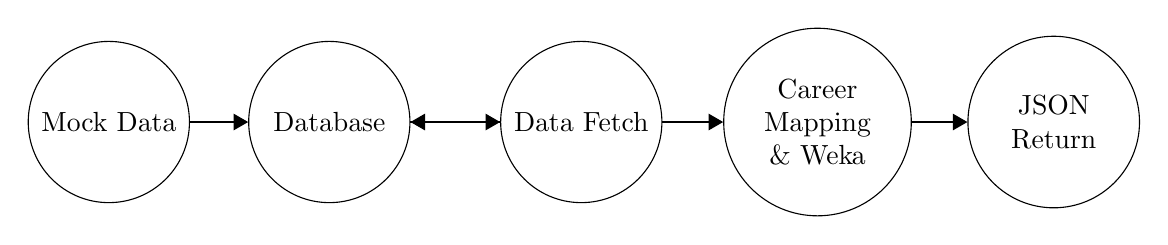
\begin{tikzpicture}[%
    >=triangle 60,              % Nice arrows; your taste may be different
    start chain=going below,    % General flow is top-to-bottom
    node distance=3mm and 20mm, % Global setup of box spacing
    every join/.style={norm},   % Default linetype for connecting boxes
    ]
% ------------------------------------------------- 
% A few box styles 
% <on chain> *and* <on grid> reduce the need for manual relative
% positioning of nodes
\tikzset{
  base/.style={draw, on chain, on grid, align=center, minimum height=2ex},
  node/.style={base, circle, text width=5em},
  % Connector line styles for different parts of the diagram
  norm/.style={->, draw},
  thin/.style={->,>=stealth',shorten >=1pt, black},
  nm/.style={->,>=stealth',shorten >=1pt, green},
  to/.style={->,>=stealth',shorten >=1pt,semithick,blue},
  thick/.style={->,shorten >=1pt,very thick, red},
  it/.style={font={\small\itshape}}
}
% -------------------------------------------------
% Start by placing the nodes
\node [node, join, xshift=-30mm] (a) {Mock Data};
\node [node, join, right = of a, xshift=8mm] (b) {Database};
\node [node, join, right = of b, xshift=12mm] (c) {Data Fetch}; 
\node [node, join, right = of c, xshift=10mm] (d) {Career Mapping \& Weka};
\node [node, join, right = of d, xshift=10mm] (e) {JSON Return};

\draw [->](c.west) |- node {} (b);

% -------------------------------------------------
\end{tikzpicture}

	\caption{High Level Architecture}
	\label{fig:HighLevelProjectArchitecture}
\end{figure}

\subsection{Overall Technology Stack}
All of the code for ProGENitor is written in Java except for the mock data
generation code which is written in Perl.  Java was selected because the code
needed to interface well with web applications and pages.  Java is easily run through
web interfaces and can easily pass data by passing JSON Objects.  Additionally,
Java interfaces well with databases.  As this project does a lot of database
scraping this was very important.
